\documentclass[10pt]{article}
\usepackage[T1]{fontenc}
\usepackage{lmodern}
\usepackage{tikz}
\usepackage[paperwidth=8.6cm,paperheight=5.45cm,margin=0cm]{geometry}

\topskip=0pt
\parindent=0pt
\pagestyle{empty}

% Strict-parsing changes relative to standard RS at the same interface.
% Points are paired means and error bars are sample SD across seeds 42--44.
% QWK is averaged over four ordinal tasks per seed; Macro-F1 is averaged over
% three binary tasks per seed. ReaSon--DS QWK is unavailable under strict parsing.
\definecolor{metricQWK}{HTML}{7A2430}
\definecolor{metricFOne}{HTML}{3F7F77}
\definecolor{gridgray}{HTML}{D6D6D6}
\definecolor{naGray}{HTML}{777777}
\definecolor{repaHighlight}{HTML}{EAF2F1}

% Panel mappings: DS [-0.40, 0.15], RF [-0.01, 0.065].
\newcommand{\dsy}[1]{0.68+(#1+0.40)*6.181818}
\newcommand{\rfy}[1]{0.68+(#1+0.01)*45.333333}

\newcommand{\dscircle}[4]{%
  \pgfmathsetmacro{\py}{\dsy{#2}}%
  \pgfmathsetmacro{\pb}{\dsy{#2-#3}}%
  \pgfmathsetmacro{\pt}{\dsy{#2+#3}}%
  \draw[metricQWK,line width=0.45pt] (#1,\pb)--(#1,\pt);
  \draw[metricQWK,line width=0.45pt] (#1-0.06,\pb)--(#1+0.06,\pb);
  \draw[metricQWK,line width=0.45pt] (#1-0.06,\pt)--(#1+0.06,\pt);
  \fill[metricQWK] (#1,\py) circle (0.065);
  \node[anchor=east,font=\sffamily\tiny,text=metricQWK]
    at (#1-0.10,\py) {#4};
}

\newcommand{\dstriangle}[4]{%
  \pgfmathsetmacro{\py}{\dsy{#2}}%
  \pgfmathsetmacro{\pb}{\dsy{#2-#3}}%
  \pgfmathsetmacro{\pt}{\dsy{#2+#3}}%
  \draw[metricFOne,line width=0.45pt] (#1,\pb)--(#1,\pt);
  \draw[metricFOne,line width=0.45pt] (#1-0.06,\pb)--(#1+0.06,\pb);
  \draw[metricFOne,line width=0.45pt] (#1-0.06,\pt)--(#1+0.06,\pt);
  \fill[metricFOne]
    (#1,\py+0.075)--(#1-0.075,\py-0.065)--(#1+0.075,\py-0.065)--cycle;
  \node[anchor=west,font=\sffamily\tiny,text=metricFOne]
    at (#1+0.10,\py) {#4};
}

\newcommand{\rfcircle}[4]{%
  \pgfmathsetmacro{\py}{\rfy{#2}}%
  \pgfmathsetmacro{\pb}{\rfy{#2-#3}}%
  \pgfmathsetmacro{\pt}{\rfy{#2+#3}}%
  \draw[metricQWK,line width=0.45pt] (#1,\pb)--(#1,\pt);
  \draw[metricQWK,line width=0.45pt] (#1-0.06,\pb)--(#1+0.06,\pb);
  \draw[metricQWK,line width=0.45pt] (#1-0.06,\pt)--(#1+0.06,\pt);
  \fill[metricQWK] (#1,\py) circle (0.065);
  \node[anchor=east,font=\sffamily\tiny,text=metricQWK]
    at (#1-0.10,\py) {#4};
}

\newcommand{\rftriangle}[4]{%
  \pgfmathsetmacro{\py}{\rfy{#2}}%
  \pgfmathsetmacro{\pb}{\rfy{#2-#3}}%
  \pgfmathsetmacro{\pt}{\rfy{#2+#3}}%
  \draw[metricFOne,line width=0.45pt] (#1,\pb)--(#1,\pt);
  \draw[metricFOne,line width=0.45pt] (#1-0.06,\pb)--(#1+0.06,\pb);
  \draw[metricFOne,line width=0.45pt] (#1-0.06,\pt)--(#1+0.06,\pt);
  \fill[metricFOne]
    (#1,\py+0.075)--(#1-0.075,\py-0.065)--(#1+0.075,\py-0.065)--cycle;
  \node[anchor=west,font=\sffamily\tiny,text=metricFOne]
    at (#1+0.10,\py) {#4};
}

\begin{document}
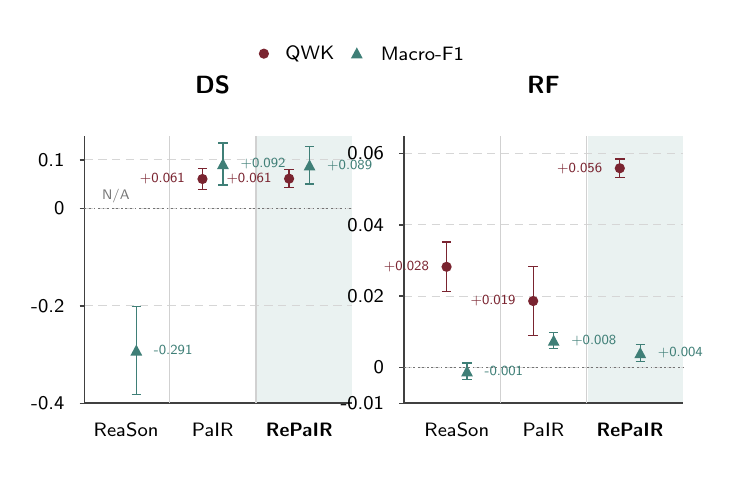
\begin{tikzpicture}[x=1cm,y=1cm,font=\sffamily]
\useasboundingbox (0,0) rectangle (8.6,5.45);

% Shared legend.
\fill[metricQWK] (3.00,5.12) circle (0.065);
\node[anchor=west,font=\sffamily\scriptsize] at (3.15,5.12) {QWK};
\fill[metricFOne]
  (4.18,5.20)--(4.105,5.06)--(4.255,5.06)--cycle;
\node[anchor=west,font=\sffamily\scriptsize] at (4.36,5.12) {Macro-F1};

\node[font=\sffamily\small\bfseries] at (2.35,4.72) {DS};
\node[font=\sffamily\small\bfseries] at (6.55,4.72) {RF};

% A pale band highlights RePaIR without changing the metric color encoding.
\fill[repaHighlight] (2.91,0.68) rectangle (4.12,4.08);
\fill[repaHighlight] (7.11,0.68) rectangle (8.32,4.08);

% DS panel: full strict range, including the ReaSon Macro-F1 drop.
\foreach \value/\label in {-0.4/{-0.4},-0.2/{-0.2},0/{0},0.1/{0.1}} {
  \pgfmathsetmacro{\gy}{\dsy{\value}}
  \draw[gridgray,densely dashed,line width=0.35pt] (0.72,\gy)--(4.12,\gy);
  \draw[black!75,line width=0.5pt] (0.66,\gy)--(0.72,\gy);
  \node[anchor=east,font=\sffamily\scriptsize] at (0.59,\gy) {\label};
}
\draw[black!75,line width=0.6pt] (0.72,0.68)--(0.72,4.08);
\draw[black!75,line width=0.6pt] (0.72,0.68)--(4.12,0.68);
\draw[black!55,densely dotted,line width=0.65pt]
  (0.72,{\dsy{0}})--(4.12,{\dsy{0}});
\draw[black!18,line width=0.4pt] (1.80,0.68)--(1.80,4.08);
\draw[black!18,line width=0.4pt] (2.90,0.68)--(2.90,4.08);

% RF panel uses a finer scale for its smaller changes.
\foreach \value/\label in {-0.01/{-0.01},0/{0},0.02/{0.02},0.04/{0.04},0.06/{0.06}} {
  \pgfmathsetmacro{\gy}{\rfy{\value}}
  \draw[gridgray,densely dashed,line width=0.35pt] (4.78,\gy)--(8.32,\gy);
  \draw[black!75,line width=0.5pt] (4.72,\gy)--(4.78,\gy);
  \node[anchor=east,font=\sffamily\scriptsize] at (4.65,\gy) {\label};
}
\draw[black!75,line width=0.6pt] (4.78,0.68)--(4.78,4.08);
\draw[black!75,line width=0.6pt] (4.78,0.68)--(8.32,0.68);
\draw[black!55,densely dotted,line width=0.65pt]
  (4.78,{\rfy{0}})--(8.32,{\rfy{0}});
\draw[black!18,line width=0.4pt] (6.00,0.68)--(6.00,4.08);
\draw[black!18,line width=0.4pt] (7.10,0.68)--(7.10,4.08);

% Method positions and labels. QWK is left, Macro-F1 is right.
\foreach \x/\name in {1.25/ReaSon,2.35/PaIR} {
  \node[anchor=north,font=\sffamily\scriptsize] at (\x,0.55) {\name};
}
\node[anchor=north,font=\sffamily\scriptsize\bfseries] at (3.45,0.55) {RePaIR};
\foreach \x/\name in {5.45/ReaSon,6.55/PaIR} {
  \node[anchor=north,font=\sffamily\scriptsize] at (\x,0.55) {\name};
}
\node[anchor=north,font=\sffamily\scriptsize\bfseries] at (7.65,0.55) {RePaIR};

% DS: method minus RS under direct-score inference.
\node[font=\sffamily\tiny,text=naGray] at (1.12,{\dsy{0.025}}) {N/A};
\dstriangle{1.38}{-0.291445}{0.090793}{-0.291}
\dscircle{2.22}{0.060740}{0.022020}{+0.061}
\dstriangle{2.48}{0.091627}{0.043052}{+0.092}
\dscircle{3.32}{0.061385}{0.018259}{+0.061}
\dstriangle{3.58}{0.088726}{0.038034}{+0.089}

% RF: method minus RS under rationale-first inference.
\rfcircle{5.32}{0.028226}{0.006966}{+0.028}
\rftriangle{5.58}{-0.001042}{0.002322}{-0.001}
\rfcircle{6.42}{0.018646}{0.009716}{+0.019}
\rftriangle{6.68}{0.007546}{0.002230}{+0.008}
\rfcircle{7.52}{0.055842}{0.002561}{+0.056}
\rftriangle{7.78}{0.004093}{0.002303}{+0.004}

\end{tikzpicture}
\end{document}
